%%%%%%%%%%%%%%%%%%%%%%%%%%%%%%%%%%%%%%% BEGINING OF A FIGURE : Allowed moves of And gadget in sliding token %%%%%%%%%%%%%%%%%%%%%%%%%%%%%%%%
\begin{figure}[H]
  \begin{subfigure}[b]{0.4\textwidth}
    \centering
    \begin{scaletikzpicturetowidth}{\textwidth}
      \begin{tikzpicture}
        \def\xa{0}
        \def\ya{0}
        %graph G
        \draw (\xa,\ya) circle (0.2cm);          %v1 no fill
        \draw (\xa,\ya+1) circle (0.2cm);        %v2 no fill
        \draw (\xa+0.5,\ya-0.8) circle (0.2cm);  %v4 no fill
        \draw (\xa-0.5,\ya-0.8) circle (0.2cm);  %v3 no fill
        \draw (\xa-1.5,\ya-1.2) circle (0.2cm);  %v5 no fill
        \draw (\xa+1.5,\ya-1.2) circle (0.2cm);  %v6 no fill
        % Tokens
        \path[fill] (\xa,\ya+1) circle (\ver);       %v2
        \path[fill] (\xa+0.5,\ya-0.8) circle (\ver); %v4
        \path[fill] (\xa-0.5,\ya-0.8) circle (\ver); %v3
        % Valid moves
        \draw[middlearrow={>}, blue] (\xa,\ya+1) -- (\xa,\ya);
        \draw[middlearrow={>}, red] (\xa-0.5,\ya-0.8) -- (\xa-1.5,\ya-1.2);
        \draw[middlearrow={>}, red] (\xa+0.5,\ya-0.8) -- (\xa+1.5,\ya-1.2);
        % paths
        \draw[thick] (\xa,\ya+1)--(\xa,\ya)--(\xa-0.5,\ya-0.8)--(\xa-1.5,\ya-1.2);
        \draw[thick] (\xa,\ya)--(\xa+0.5,\ya-0.8)--(\xa+1.5,\ya-1.2);
        \path[draw, thick, dashed, rounded corners=4mm] (\xa,\ya+0.6)--(\xa+1.2,\ya-1.2)--(\xa-1.2,\ya-1.2)--cycle;
      \end{tikzpicture}
    \end{scaletikzpicturetowidth}
    \caption{$AND$}
    \label{fig:and_valid_move_NCL}
  \end{subfigure}
  \hspace{3em} % vertical space
  \begin{subfigure}[b]{0.4\textwidth}
    \centering
    \begin{scaletikzpicturetowidth}{\textwidth}
      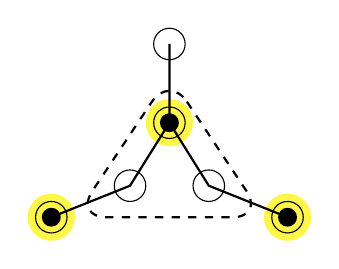
\begin{tikzpicture}
        \def\xb{5}
        \def\yb{0}
        % Highlight change
        \draw[fill=yellow, opacity=.7, draw=none] (\xb,\yb) circle (0.3cm);
        \draw[fill=yellow, opacity=.7, draw=none] (\xb-1.5,\yb-1.2) circle (0.3cm);
        \draw[fill=yellow, opacity=.7, draw=none] (\xb+1.5,\yb-1.2)  circle (0.3cm);

        %graph G : token slide
        \draw (\xb,\yb) circle (0.2cm);          %v1 no fill
        \draw (\xb,\yb+1) circle (0.2cm);        %v2 no fill
        \draw (\xb+0.5,\yb-0.8) circle (0.2cm);  %v4 no fill
        \draw (\xb-0.5,\yb-0.8) circle (0.2cm);  %v3 no fill
        \draw (\xb-1.5,\yb-1.2) circle (0.2cm);  %v5 no fill
        \draw (\xb+1.5,\yb-1.2) circle (0.2cm);  %v6 no fill

        \path[fill] (\xb,\yb) circle (\ver);         %v1
        \path[fill] (\xb-1.5,\yb-1.2) circle (\ver); %v5
        \path[fill] (\xb+1.5,\yb-1.2) circle (\ver); %v6
        %labels
        \draw[thick] (\xb,\yb+1)--(\xb,\yb)--(\xb-0.5,\yb-0.8)--(\xb-1.5,\yb-1.2);
        \draw[thick] (\xb,\yb)--(\xb+0.5,\yb-0.8)--(\xb+1.5,\yb-1.2);
        \path[draw, thick, dashed, rounded corners=4mm] (\xb,\yb+0.6)--(\xb+1.2,\yb-1.2)--(\xb-1.2,\yb-1.2)--cycle;
      \end{tikzpicture}
    \end{scaletikzpicturetowidth}
    \caption{$AND$}
    \label{fig:and_valid_move_NCL_changed}
  \end{subfigure}
  \caption{Valid move of AND gadget.}
  \label{fig:and}
\end{figure}
%%%%%%%%%%%%%%%%%%%%%%%%%%%%%%%%%%%%%%%%%%%%%%%% ENDING OF A FIGURE %%%%%%%%%%%%%%%%%%%%%%%%%%%%%%%%%%%%%%%%%%%%%%%%

%%%%%%%%%%%%%%%%%%%%%%%%%%%%%%%%%%%%%%%%%%%%%%%% BEGINING OF A FIGURE : Allowed moves of OR gadget %%%%%%%%%%%%%%%%%%%%%%%%%%%%%%%%%%%%%%%%%%%%%%%
\begin{figure}[H]
  \begin{subfigure}[b]{0.4\textwidth}
    \centering
    \begin{scaletikzpicturetowidth}{\textwidth}
      \begin{tikzpicture}
        \def\xb{0}
        \def\yb{0}
        %G_1
        \draw (\xb,\yb+2) circle (0.2cm);         %v9
        \draw (\xb,\yb) circle (0.2cm);           %v1
        \draw (\xb+0.5,\yb-0.8) circle (0.2cm);   %v4
        \draw (\xb-0.5,\yb-0.8) circle (0.2cm);   %v3
        \draw (\xb,\yb+1) circle (0.2cm);         %v2
        \draw (\xb-1.5,\yb-1.5) circle (0.2cm);   %v5
        \draw (\xb+1.5,\yb-1.5) circle (0.2cm);   %v6
        \draw (\xb-2.5,\yb-2.2) circle (0.2cm);     %v7
        \draw (\xb+2.5,\yb-2.2) circle (0.2cm);     %v8
        % Tokens
        \path[fill] (\xb,\yb+2) circle (\ver);         %v0
        \path[fill] (\xb,\yb) circle (\ver);           %v1
        \path[fill] (\xb-1.5,\yb-1.5) circle (\ver);   %v5
        \path[fill] (\xb+1.5,\yb-1.5) circle (\ver);   %v6
        % valid moves
        \draw[middlearrow={>}, blue] (\xb,\yb+2) -- (\xb,\yb+1);
        \draw[middlearrow={>}, blue] (\xb,\yb) -- (\xb-0.5,\yb-0.8);
        \draw[middlearrow={>}, blue] (\xb-1.5,\yb-1.5) -- (\xb-2.5,\yb-2.2);
        %paths
        \draw[thick] (\xb,\yb+2)--(\xb,\yb+1)--(\xb,\yb)--(\xb-0.5,\yb-0.8)--(\xb-1.5,\yb-1.5)--(\xb-2.5,\yb-2.2);
        \draw[thick] (\xb,\yb)--(\xb+0.5,\yb-0.8)--(\xb+1.5,\yb-1.5)--(\xb+2.5,\yb-2.2);
        \draw[thick] (\xb-0.5,\yb-0.8)--(\xb+0.5,\yb-0.8);
        \path[draw, thick, dashed, rounded corners=6mm] (\xb,\yb+1.8)--(\xb+2.2,\yb-2)--(\xb-2.2,\yb-2)--cycle;
      \end{tikzpicture}
    \end{scaletikzpicturetowidth}
    \caption{$OR$}
    \label{fig:or_valid_move_NCL}
  \end{subfigure}
  \hspace{3em} % vertical space
  \begin{subfigure}[b]{0.4\textwidth}
    \centering
    \begin{scaletikzpicturetowidth}{\textwidth}
      \begin{tikzpicture}
        \def\xc{0}
        \def\yc{0}
        %G_2
        \draw (\xc,\yc+2) circle (0.2cm);         %v9
        \draw (\xc,\yc) circle (0.2cm);           %v1
        \draw (\xc+0.5,\yc-0.8) circle (0.2cm);   %v4
        \draw (\xc-0.5,\yc-0.8) circle (0.2cm);   %v3
        \draw (\xc,\yc+1) circle (0.2cm);         %v2
        \draw (\xc-1.5,\yc-1.5) circle (0.2cm);   %v5
        \draw (\xc+1.5,\yc-1.5) circle (0.2cm);   %v6
        \draw (\xc-2.5,\yc-2.2) circle (0.2cm);     %v7
        \draw (\xc+2.5,\yc-2.2) circle (0.2cm);     %v8
        % Tokens
        \path[fill] (\xc,\yc+2) circle (\ver);         %v0
        \path[fill] (\xc,\yc) circle (\ver);           %v1
        \path[fill] (\xc-1.5,\yc-1.5) circle (\ver);   %v5
        \path[fill] (\xc+1.5,\yc-1.5) circle (\ver);   %v6
        % valid moves
        \draw[middlearrow={>}, blue] (\xc,\yc+2) -- (\xc,\yc+1);
        \draw[middlearrow={>}, blue] (\xc,\yc) -- (\xc+0.5,\yc-0.8);
        \draw[middlearrow={>}, blue] (\xc+1.5,\yc-1.5) -- (\xc+2.5,\yc-2.2);
        %paths
        \draw[thick] (\xc,\yc+2)--(\xc,\yc+1)--(\xc,\yc)--(\xc-0.5,\yc-0.8)--(\xc-1.5,\yc-1.5)--(\xc-2.5,\yc-2.2);
        \draw[thick] (\xc,\yc)--(\xc+0.5,\yc-0.8)--(\xc+1.5,\yc-1.5)--(\xc+2.5,\yc-2.2);
        \draw[thick] (\xc-0.5,\yc-0.8)--(\xc+0.5,\yc-0.8);
        \path[draw, thick, dashed, rounded corners=6mm] (\xc,\yc+1.8)--(\xc+2.2,\yc-2)--(\xc-2.2,\yc-2)--cycle;
      \end{tikzpicture}
    \end{scaletikzpicturetowidth}
    \caption{$OR$}
    \label{fig:or_valid_move_NCL_changed}
  \end{subfigure}
  \caption{Valid moves of an $OR$ gadget.}
  \label{fig:or}
\end{figure}
%%%%%%%%%%%%%%%%%%%%%%%%%%%%%%%%%%%%%%%%%%%%%%%% ENDING OF A FIGURE %%%%%%%%%%%%%%%%%%%%%%%%%%%%%%%%%%%%%%%%%%%%%%%%

\begin{figure}[H]
  \begin{subfigure}[b]{0.4\textwidth}
    \centering
    \begin{scaletikzpicturetowidth}{\textwidth}
      \begin{tikzpicture}
        \def\ver{0.15} %size of a vertex
        % v1
        \def\xa{0}
        \def\ya{0}
        %----------------- arrrows -----------------
        \node (1) at (\xa+5,\ya) {$\Rightarrow$};
        %----------------- arrrows -----------------
        % f_1 arrows
        \draw[middlearrow={<}, red] (\xa-2,\ya+1.5)-- (\xa+2,\ya+1.5);        % v2 - v3
        \draw[middlearrow={<}, red] (\xa+2,\ya+1.5) -- (\xa,\ya);             % v3 - v1
        \draw[middlearrow={<}, red] (\xa,\ya) -- (\xa-2,\ya+1.5);             % v1 - v2
        \draw[middlearrow={<}, blue] (\xa-2,\ya+1.5) -- (\xa-2,\ya-3.5);      % v2 - v4
        \draw[middlearrow={<}, blue] (\xa,\ya) -- (\xa,\ya-2);                % v1 - v6
        \draw[middlearrow={<}, blue] (\xa+2,\ya+1.5) -- (\xa+2,\ya-3.5);      % v3 - v5
        \draw[middlearrow={>}, blue] (\xa-2,\ya-3.5) -- (\xa+2,\ya-3.5);      % v4 - v5
        \draw[middlearrow={<}, blue] (\xa-2,\ya-3.5) -- (\xa,\ya-2);          % v4 - v6
        \draw[middlearrow={<}, blue] (\xa,\ya-2) -- (\xa+2,\ya-3.5);          % v6 - v5

        \draw[ultra thick, -, red] (\xa-2,\ya+1.5) -- (\xa+2,\ya+1.5);       % v2 - v3
        \draw[ultra thick, -, red] (\xa+2,\ya+1.5) -- (\xa,\ya);             % v3 - v1
        \draw[ultra thick, -, red] (\xa,\ya) -- (\xa-2,\ya+1.5);             % v1 - v2
        \draw[ultra thick, -, blue] (\xa-2,\ya+1.5) -- (\xa-2,\ya-3.5);      % v2 - v4
        \draw[ultra thick, -, blue] (\xa,\ya) -- (\xa,\ya-2);                % v1 - v6
        \draw[ultra thick, -, blue] (\xa+2,\ya+1.5) -- (\xa+2,\ya-3.5);      % v3 - v5
        \draw[ultra thick, -, blue] (\xa-2,\ya-3.5) -- (\xa+2,\ya-3.5);      % v4 - v5
        \draw[ultra thick, -, blue] (\xa-2,\ya-3.5) -- (\xa,\ya-2);          % v4 - v6
        \draw[ultra thick, -, blue] (\xa,\ya-2) -- (\xa+2,\ya-3.5);          % v6 - v5

        %graph G : Nodes fill
        \path[fill] (\xa,\ya) circle (\ver);           %v1
        \path[fill] (\xa-2,\ya+1.5) circle (\ver);   %v2
        \path[fill] (\xa+2,\ya+1.5) circle (\ver);   %v3
        \path[fill] (\xa-2,\ya-3.5) circle (\ver);   %v4
        \path[fill] (\xa+2,\ya-3.5) circle (\ver);   %v5
        \path[fill] (\xa,\ya-2) circle (\ver);         %v6
      \end{tikzpicture}
    \end{scaletikzpicturetowidth}
    \caption{$OR$}
    \label{fig:instance}
  \end{subfigure}
  \hspace{3em} % vertical space
  \begin{subfigure}[b]{0.4\textwidth}
    \centering
    \begin{scaletikzpicturetowidth}{\textwidth}
      \begin{tikzpicture}
        \def\ver{0.15} %size of a vertex
        % v1
        \def\xa{0}
        \def\ya{0}
        % Highlight change
        \draw[fill=yellow, opacity=.7, ultra thick, dotted, rotate around={90:(\xa,\ya+1.5)},yellow] (\xa,\ya+1.5) ellipse (10pt and 65pt);
        % f_1 arrows
        \draw[middlearrow={>}, red] (\xa-2,\ya+1.5)-- (\xa+2,\ya+1.5);        % v2 - v3
        \draw[middlearrow={<}, red] (\xa+2,\ya+1.5) -- (\xa,\ya);             % v3 - v1
        \draw[middlearrow={<}, red] (\xa,\ya) -- (\xa-2,\ya+1.5);             % v1 - v2
        \draw[middlearrow={<}, blue] (\xa-2,\ya+1.5) -- (\xa-2,\ya-3.5);      % v2 - v4
        \draw[middlearrow={<}, blue] (\xa,\ya) -- (\xa,\ya-2);                % v1 - v6
        \draw[middlearrow={<}, blue] (\xa+2,\ya+1.5) -- (\xa+2,\ya-3.5);      % v3 - v5
        \draw[middlearrow={>}, blue] (\xa-2,\ya-3.5) -- (\xa+2,\ya-3.5);      % v4 - v5
        \draw[middlearrow={<}, blue] (\xa-2,\ya-3.5) -- (\xa,\ya-2);          % v4 - v6
        \draw[middlearrow={<}, blue] (\xa,\ya-2) -- (\xa+2,\ya-3.5);          % v6 - v5

        \draw[ultra thick, -, red] (\xa-2,\ya+1.5) -- (\xa+2,\ya+1.5);       % v2 - v3
        \draw[ultra thick, -, red] (\xa+2,\ya+1.5) -- (\xa,\ya);             % v3 - v1
        \draw[ultra thick, -, red] (\xa,\ya) -- (\xa-2,\ya+1.5);             % v1 - v2
        \draw[ultra thick, -, blue] (\xa-2,\ya+1.5) -- (\xa-2,\ya-3.5);      % v2 - v4
        \draw[ultra thick, -, blue] (\xa,\ya) -- (\xa,\ya-2);                % v1 - v6
        \draw[ultra thick, -, blue] (\xa+2,\ya+1.5) -- (\xa+2,\ya-3.5);      % v3 - v5
        \draw[ultra thick, -, blue] (\xa-2,\ya-3.5) -- (\xa+2,\ya-3.5);      % v4 - v5
        \draw[ultra thick, -, blue] (\xa-2,\ya-3.5) -- (\xa,\ya-2);          % v4 - v6
        \draw[ultra thick, -, blue] (\xa,\ya-2) -- (\xa+2,\ya-3.5);          % v6 - v5

        %graph G : Nodes fill
        \path[fill] (\xa,\ya) circle (\ver);           %v1
        \path[fill] (\xa-2,\ya+1.5) circle (\ver);   %v2
        \path[fill] (\xa+2,\ya+1.5) circle (\ver);   %v3
        \path[fill] (\xa-2,\ya-3.5) circle (\ver);   %v4
        \path[fill] (\xa+2,\ya-3.5) circle (\ver);   %v5
        \path[fill] (\xa,\ya-2) circle (\ver);         %v6

      \end{tikzpicture}
    \end{scaletikzpicturetowidth}
    \caption{$OR$}
    \label{fig:input_instance_1}
  \end{subfigure}
  \hspace{3em} % vertical space
  \begin{subfigure}[b]{0.4\textwidth}
    \centering
    \begin{scaletikzpicturetowidth}{\textwidth}
      \begin{tikzpicture}
        \def\ver{0.15} %size of a vertex
        % v1
        \def\xa{0}
        \def\ya{0}
        % Highlight change
        \draw[fill=yellow, opacity=.7, ultra thick, dotted, rotate around={305:(\xa+1,\ya+0.75)},yellow] (\xa+1,\ya+0.75) ellipse (10pt and 45pt);
        % f_1 arrows
        \draw[middlearrow={>}, red] (\xa-2,\ya+1.5)-- (\xa+2,\ya+1.5);        % v2 - v3
        \draw[middlearrow={>}, red] (\xa+2,\ya+1.5) -- (\xa,\ya);             % v3 - v1
        \draw[middlearrow={<}, red] (\xa,\ya) -- (\xa-2,\ya+1.5);             % v1 - v2
        \draw[middlearrow={<}, blue] (\xa-2,\ya+1.5) -- (\xa-2,\ya-3.5);      % v2 - v4
        \draw[middlearrow={<}, blue] (\xa,\ya) -- (\xa,\ya-2);                % v1 - v6
        \draw[middlearrow={<}, blue] (\xa+2,\ya+1.5) -- (\xa+2,\ya-3.5);      % v3 - v5
        \draw[middlearrow={>}, blue] (\xa-2,\ya-3.5) -- (\xa+2,\ya-3.5);      % v4 - v5
        \draw[middlearrow={<}, blue] (\xa-2,\ya-3.5) -- (\xa,\ya-2);          % v4 - v6
        \draw[middlearrow={<}, blue] (\xa,\ya-2) -- (\xa+2,\ya-3.5);          % v6 - v5

        \draw[ultra thick, -, red] (\xa-2,\ya+1.5) -- (\xa+2,\ya+1.5);       % v2 - v3
        \draw[ultra thick, -, red] (\xa+2,\ya+1.5) -- (\xa,\ya);             % v3 - v1
        \draw[ultra thick, -, red] (\xa,\ya) -- (\xa-2,\ya+1.5);             % v1 - v2
        \draw[ultra thick, -, blue] (\xa-2,\ya+1.5) -- (\xa-2,\ya-3.5);      % v2 - v4
        \draw[ultra thick, -, blue] (\xa,\ya) -- (\xa,\ya-2);                % v1 - v6
        \draw[ultra thick, -, blue] (\xa+2,\ya+1.5) -- (\xa+2,\ya-3.5);      % v3 - v5
        \draw[ultra thick, -, blue] (\xa-2,\ya-3.5) -- (\xa+2,\ya-3.5);      % v4 - v5
        \draw[ultra thick, -, blue] (\xa-2,\ya-3.5) -- (\xa,\ya-2);          % v4 - v6
        \draw[ultra thick, -, blue] (\xa,\ya-2) -- (\xa+2,\ya-3.5);          % v6 - v5

        %graph G : Nodes fill
        \path[fill] (\xa,\ya) circle (\ver);           %v1
        \path[fill] (\xa-2,\ya+1.5) circle (\ver);   %v2
        \path[fill] (\xa+2,\ya+1.5) circle (\ver);   %v3
        \path[fill] (\xa-2,\ya-3.5) circle (\ver);   %v4
        \path[fill] (\xa+2,\ya-3.5) circle (\ver);   %v5
        \path[fill] (\xa,\ya-2) circle (\ver);         %v6

      \end{tikzpicture}
    \end{scaletikzpicturetowidth}
    \caption{$OR$}
    \label{fig:input_instance_2}
  \end{subfigure}
  \hspace{3em} % vertical space
  \begin{subfigure}[b]{0.4\textwidth}
    \centering
    \begin{scaletikzpicturetowidth}{\textwidth}
      \begin{tikzpicture}
        \def\ver{0.15} %size of a vertex
        % v1
        \def\xa{0}
        \def\ya{0}
        % Highlight change
        \draw[fill=yellow, opacity=.7, ultra thick, dotted, rotate around={180:(\xa,\ya-1)},yellow] (\xa,\ya-1) ellipse (10pt and 45pt);
        % f_1 arrows
        \draw[middlearrow={>}, red] (\xa-2,\ya+1.5)-- (\xa+2,\ya+1.5);        % v2 - v3
        \draw[middlearrow={>}, red] (\xa+2,\ya+1.5) -- (\xa,\ya);             % v3 - v1
        \draw[middlearrow={<}, red] (\xa,\ya) -- (\xa-2,\ya+1.5);             % v1 - v2
        \draw[middlearrow={<}, blue] (\xa-2,\ya+1.5) -- (\xa-2,\ya-3.5);      % v2 - v4
        \draw[middlearrow={>}, blue] (\xa,\ya) -- (\xa,\ya-2);                % v1 - v6
        \draw[middlearrow={<}, blue] (\xa+2,\ya+1.5) -- (\xa+2,\ya-3.5);      % v3 - v5
        \draw[middlearrow={>}, blue] (\xa-2,\ya-3.5) -- (\xa+2,\ya-3.5);      % v4 - v5
        \draw[middlearrow={<}, blue] (\xa-2,\ya-3.5) -- (\xa,\ya-2);          % v4 - v6
        \draw[middlearrow={<}, blue] (\xa,\ya-2) -- (\xa+2,\ya-3.5);          % v6 - v5

        \draw[ultra thick, -, red] (\xa-2,\ya+1.5) -- (\xa+2,\ya+1.5);       % v2 - v3
        \draw[ultra thick, -, red] (\xa+2,\ya+1.5) -- (\xa,\ya);             % v3 - v1
        \draw[ultra thick, -, red] (\xa,\ya) -- (\xa-2,\ya+1.5);             % v1 - v2
        \draw[ultra thick, -, blue] (\xa-2,\ya+1.5) -- (\xa-2,\ya-3.5);      % v2 - v4
        \draw[ultra thick, -, blue] (\xa,\ya) -- (\xa,\ya-2);                % v1 - v6
        \draw[ultra thick, -, blue] (\xa+2,\ya+1.5) -- (\xa+2,\ya-3.5);      % v3 - v5
        \draw[ultra thick, -, blue] (\xa-2,\ya-3.5) -- (\xa+2,\ya-3.5);      % v4 - v5
        \draw[ultra thick, -, blue] (\xa-2,\ya-3.5) -- (\xa,\ya-2);          % v4 - v6
        \draw[ultra thick, -, blue] (\xa,\ya-2) -- (\xa+2,\ya-3.5);          % v6 - v5

        %graph G : Nodes fill
        \path[fill] (\xa,\ya) circle (\ver);           %v1
        \path[fill] (\xa-2,\ya+1.5) circle (\ver);   %v2
        \path[fill] (\xa+2,\ya+1.5) circle (\ver);   %v3
        \path[fill] (\xa-2,\ya-3.5) circle (\ver);   %v4
        \path[fill] (\xa+2,\ya-3.5) circle (\ver);   %v5
        \path[fill] (\xa,\ya-2) circle (\ver);         %v6

      \end{tikzpicture}
    \end{scaletikzpicturetowidth}
    \caption{$OR$}
    \label{fig:input_instance_3}
  \end{subfigure}
  \caption{Sliding Tokens vertex gadgets.}
  \label{fig:input_instance_config_to_edge}
\end{figure}


\paragraph{Output Sliding-Token instance}
%%%%%%%%%%%%%%%%%%%%%%%%%%%%%%%%%%%%%%%%%%%%%%%% BEGINING OF A FIGURE : Initital AND/OR gadget graph  %%%%%%%%%%%%%%%%%%%%%%%%%%%%%%%%%%%%%%%%%%%%%%%
\begin{figure}[H]
  \centering
  \begin{scaletikzpicturetowidth}{\textwidth}
    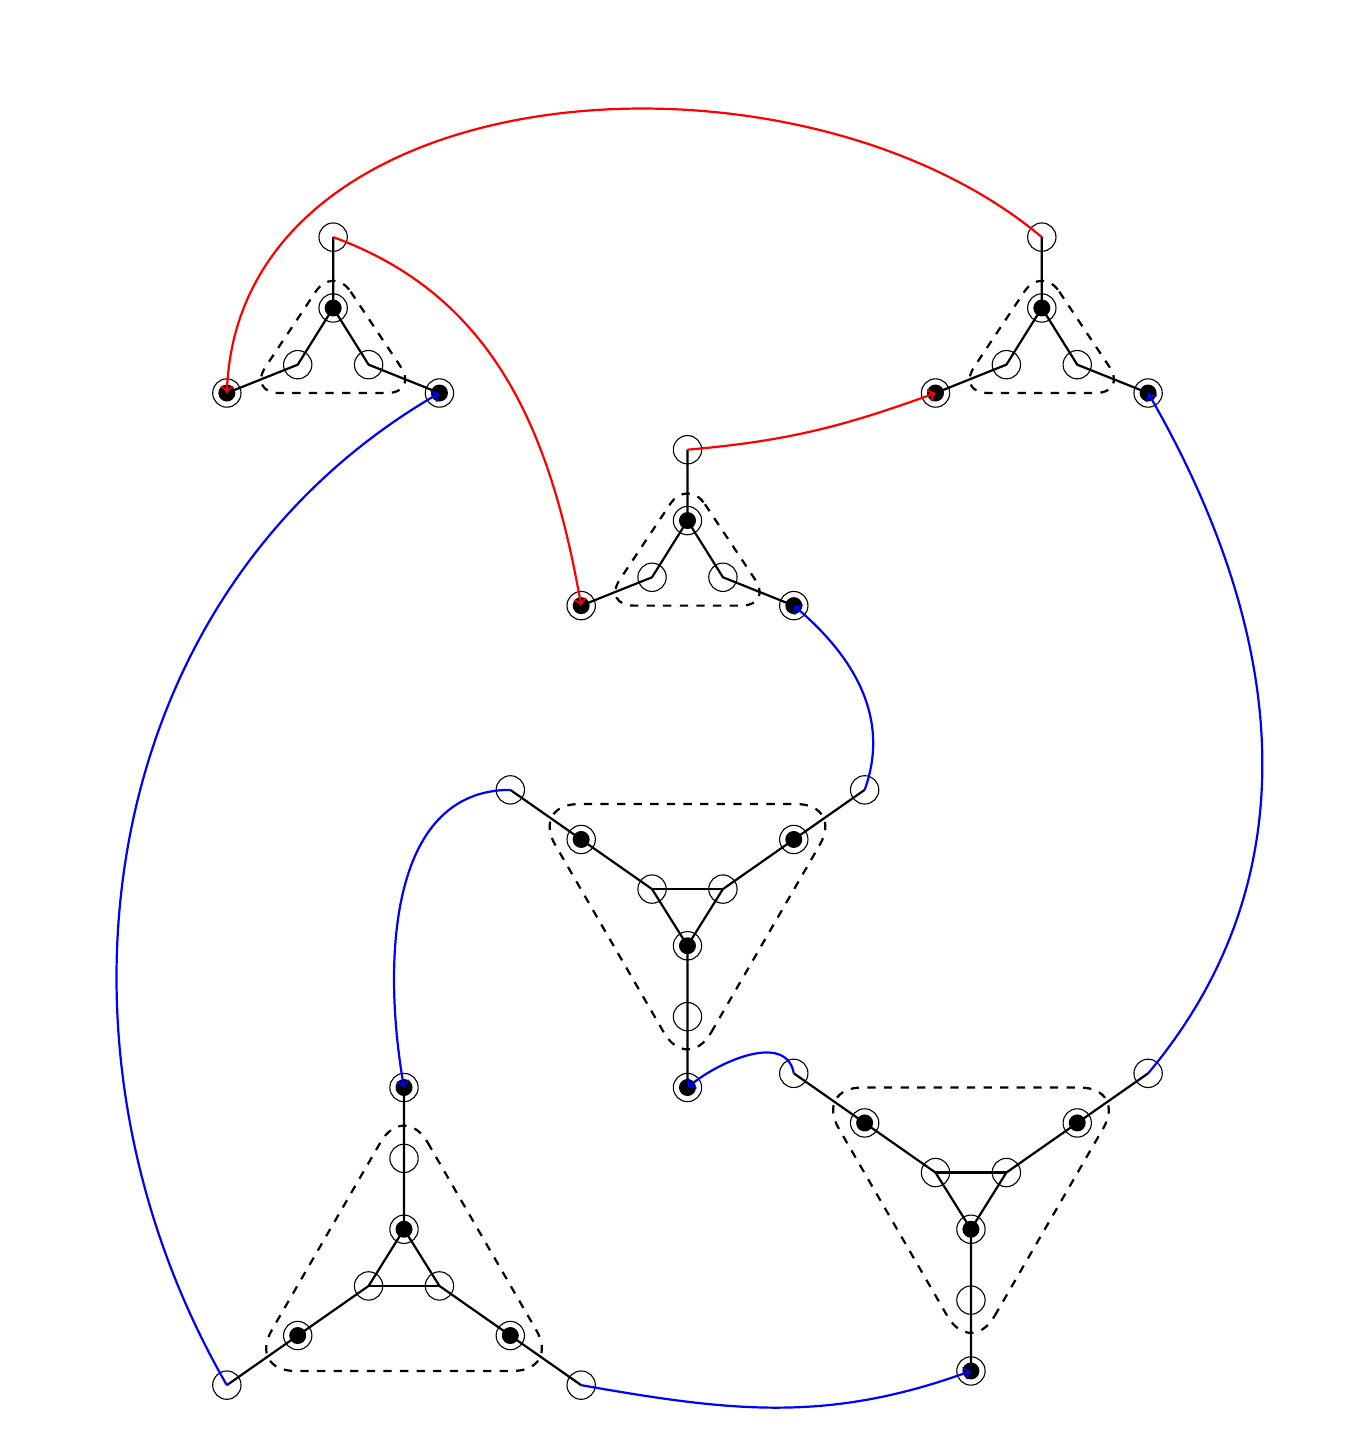
\begin{tikzpicture}[scale=0.9]
      %%%%%%%%%%%% AND 1 %%%%%%%%%%%%
      \def\ver{0.12} %size of a vertex
      \def\xa{-1}
      \def\ya{0}
      %graph G
      \draw (\xa,\ya) circle (0.2cm);          %v1 no fill
      \draw (\xa,\ya+1) circle (0.2cm);        %v2 no fill
      \draw (\xa+0.5,\ya-0.8) circle (0.2cm);  %v4 no fill
      \draw (\xa-0.5,\ya-0.8) circle (0.2cm);  %v3 no fill
      \draw (\xa-1.5,\ya-1.2) circle (0.2cm);  %v5 no fill
      \draw (\xa+1.5,\ya-1.2) circle (0.2cm);  %v6 no fill
      \path[fill] (\xa,\ya) circle (\ver);        %v1
      \path[fill] (\xa-1.5,\ya-1.2) circle (\ver); %v5
      \path[fill] (\xa+1.5,\ya-1.2) circle (\ver);%v6
      %labels
      \draw[thick] (\xa,\ya+1)--(\xa,\ya)--(\xa-0.5,\ya-0.8)--(\xa-1.5,\ya-1.2);
      \draw[thick] (\xa,\ya)--(\xa+0.5,\ya-0.8)--(\xa+1.5,\ya-1.2);
      \path[draw, thick, dashed, rounded corners=4mm] (\xa,\ya+0.6)--(\xa+1.2,\ya-1.2)--(\xa-1.2,\ya-1.2)--cycle;

      %%%%%%%%%%%% AND 2 %%%%%%%%%%%%
      \def\ver{0.12} %size of a vertex
      \def\xb{4}
      \def\yb{-3}
      %graph G
      \draw (\xb,\yb) circle (0.2cm);          %v1 no fill
      \draw (\xb,\yb+1) circle (0.2cm);        %v2 no fill
      \draw (\xb+0.5,\yb-0.8) circle (0.2cm);  %v4 no fill
      \draw (\xb-0.5,\yb-0.8) circle (0.2cm);  %v3 no fill
      \draw (\xb-1.5,\yb-1.2) circle (0.2cm);  %v5 no fill
      \draw (\xb+1.5,\yb-1.2) circle (0.2cm);  %v6 no fill
      \path[fill] (\xb,\yb) circle (\ver);       %v1
      \path[fill] (\xb-1.5,\yb-1.2) circle (\ver); %v5
      \path[fill] (\xb+1.5,\yb-1.2) circle (\ver); %v6
      %labels
      \draw[thick] (\xb,\yb+1)--(\xb,\yb)--(\xb-0.5,\yb-0.8)--(\xb-1.5,\yb-1.2);
      \draw[thick] (\xb,\yb)--(\xb+0.5,\yb-0.8)--(\xb+1.5,\yb-1.2);
      \path[draw, thick, dashed, rounded corners=4mm] (\xb,\yb+0.6)--(\xb+1.2,\yb-1.2)--(\xb-1.2,\yb-1.2)--cycle;

      %%%%%%%%%%%% AND 3 %%%%%%%%%%%%
      \def\ver{0.12} %size of a vertex
      \def\xc{9}
      \def\yc{0}
      %graph G
      \draw (\xc,\yc) circle (0.2cm);          %v1 no fill
      \draw (\xc,\yc+1) circle (0.2cm);        %v2 no fill
      \draw (\xc+0.5,\yc-0.8) circle (0.2cm);  %v4 no fill
      \draw (\xc-0.5,\yc-0.8) circle (0.2cm);  %v3 no fill
      \draw (\xc-1.5,\yc-1.2) circle (0.2cm);  %v5 no fill
      \draw (\xc+1.5,\yc-1.2) circle (0.2cm);  %v6 no fill
      \path[fill] (\xc,\yc) circle (\ver);       %v1
      \path[fill] (\xc-1.5,\yc-1.2) circle (\ver); %v5
      \path[fill] (\xc+1.5,\yc-1.2) circle (\ver); %v6
      %labels
      \draw[thick] (\xc,\yc+1)--(\xc,\yc)--(\xc-0.5,\yc-0.8)--(\xc-1.5,\yc-1.2);
      \draw[thick] (\xc,\yc)--(\xc+0.5,\yc-0.8)--(\xc+1.5,\yc-1.2);
      \path[draw, thick, dashed, rounded corners=4mm] (\xc,\yc+0.6)--(\xc+1.2,\yc-1.2)--(\xc-1.2,\yc-1.2)--cycle;

      %%%%%%%%%%%% OR 1 %%%%%%%%%%%%
      \def\ver{0.12} %size of a vertex
      \def\xd{0}
      \def\yd{-13}
      %G_1
      \draw (\xd,\yd+2) circle (0.2cm);         %v9
      \draw (\xd,\yd) circle (0.2cm);           %v1
      \draw (\xd+0.5,\yd-0.8) circle (0.2cm);   %v4
      \draw (\xd-0.5,\yd-0.8) circle (0.2cm);   %v3
      \draw (\xd,\yd+1) circle (0.2cm);         %v2
      \draw (\xd-1.5,\yd-1.5) circle (0.2cm);   %v5
      \draw (\xd+1.5,\yd-1.5) circle (0.2cm);   %v6
      \draw (\xd-2.5,\yd-2.2) circle (0.2cm);     %v7
      \draw (\xd+2.5,\yd-2.2) circle (0.2cm);     %v8

      \path[fill] (\xd,\yd+2) circle (\ver);         %v0
      \path[fill] (\xd,\yd) circle (\ver);           %v1
      \path[fill] (\xd-1.5,\yd-1.5) circle (\ver);   %v5
      \path[fill] (\xd+1.5,\yd-1.5) circle (\ver);   %v6
      %labels
      \draw[thick] (\xd,\yd+2)--(\xd,\yd+1)--(\xd,\yd)--(\xd-0.5,\yd-0.8)--(\xd-1.5,\yd-1.5)--(\xd-2.5,\yd-2.2);
      \draw[thick] (\xd,\yd)--(\xd+0.5,\yd-0.8)--(\xd+1.5,\yd-1.5)--(\xd+2.5,\yd-2.2);
      \draw[thick] (\xd-0.5,\yd-0.8)--(\xd+0.5,\yd-0.8);
      \path[draw, thick, dashed, rounded corners=6mm] (\xd,\yd+1.8)--(\xd+2.2,\yd-2)--(\xd-2.2,\yd-2)--cycle;

      %%%%%%%%%%%% OR 2 %%%%%%%%%%%%
      \def\ver{0.12} %size of a vertex
      \def\xe{4}
      \def\ye{-9}
      %G_1
      \draw (\xe,\ye-2) circle (0.2cm);         %v9
      \draw (\xe,\ye) circle (0.2cm);           %v1
      \draw (\xe+0.5,\ye+0.8) circle (0.2cm);   %v4
      \draw (\xe-0.5,\ye+0.8) circle (0.2cm);   %v3
      \draw (\xe,\ye-1) circle (0.2cm);         %v2
      \draw (\xe-1.5,\ye+1.5) circle (0.2cm);   %v5
      \draw (\xe+1.5,\ye+1.5) circle (0.2cm);   %v6
      \draw (\xe-2.5,\ye+2.2) circle (0.2cm);     %v7
      \draw (\xe+2.5,\ye+2.2) circle (0.2cm);     %v8

      \path[fill] (\xe,\ye-2) circle (\ver);         %v0
      \path[fill] (\xe,\ye) circle (\ver);           %v1
      \path[fill] (\xe-1.5,\ye+1.5) circle (\ver);   %v5
      \path[fill] (\xe+1.5,\ye+1.5) circle (\ver);   %v6
      %labels
      \draw[thick] (\xe,\ye-2)--(\xe,\ye-1)--(\xe,\ye)--(\xe-0.5,\ye+0.8)--(\xe-1.5,\ye+1.5)--(\xe-2.5,\ye+2.2);
      \draw[thick] (\xe,\ye)--(\xe+0.5,\ye+0.8)--(\xe+1.5,\ye+1.5)--(\xe+2.5,\ye+2.2);
      \draw[thick] (\xe-0.5,\ye+0.8)--(\xe+0.5,\ye+0.8);
      \path[draw, thick, dashed, rounded corners=6mm] (\xe,\ye-1.8)--(\xe+2.2,\ye+2)--(\xe-2.2,\ye+2)--cycle;

      %%%%%%%%%%%% OR 3 %%%%%%%%%%%%
      \def\ver{0.12} %size of a vertex
      \def\xf{8}
      \def\yf{-13}
      %G_1
      \draw (\xf,\yf-2) circle (0.2cm);         %v9
      \draw (\xf,\yf) circle (0.2cm);           %v1
      \draw (\xf+0.5,\yf+0.8) circle (0.2cm);   %v4
      \draw (\xf-0.5,\yf+0.8) circle (0.2cm);   %v3
      \draw (\xf,\yf-1) circle (0.2cm);         %v2
      \draw (\xf-1.5,\yf+1.5) circle (0.2cm);   %v5
      \draw (\xf+1.5,\yf+1.5) circle (0.2cm);   %v6
      \draw (\xf-2.5,\yf+2.2) circle (0.2cm);     %v7
      \draw (\xf+2.5,\yf+2.2) circle (0.2cm);     %v8

      \path[fill] (\xf,\yf-2) circle (\ver);         %v0
      \path[fill] (\xf,\yf) circle (\ver);           %v1
      \path[fill] (\xf-1.5,\yf+1.5) circle (\ver);   %v5
      \path[fill] (\xf+1.5,\yf+1.5) circle (\ver);   %v6
      %labels
      \draw[thick] (\xf,\yf-2)--(\xf,\yf-1)--(\xf,\yf)--(\xf-0.5,\yf+0.8)--(\xf-1.5,\yf+1.5)--(\xf-2.5,\yf+2.2);
      \draw[thick] (\xf,\yf)--(\xf+0.5,\yf+0.8)--(\xf+1.5,\yf+1.5)--(\xf+2.5,\yf+2.2);
      \draw[thick] (\xf-0.5,\yf+0.8)--(\xf+0.5,\yf+0.8);
      \path[draw, thick, dashed, rounded corners=6mm] (\xf,\yf-1.8)--(\xf+2.2,\yf+2)--(\xf-2.2,\yf+2)--cycle;

      %%%%%%%%%%% EDGES %%%%%%%%%
      \draw [-, red, thick, arrows={->[scale=3,red]}] (\xc,\yc+1) to [out=140,in=88] (\xa-1.5,\ya-1.2);              % AND 3  -- AND 1
      \draw [-, red, thick, arrows={->[scale=3,red]}] (\xa,\ya+1) to [out=340,in=100] (\xb-1.5,\yb-1.2);             % AND 1  -- AND 2
      \draw [-, red, thick, arrows={->[scale=3,red]}] (\xb,\yb+1) to [out=5,in=200] (\xc-1.5,\yc-1.2);              % AND 2  -- AND 3
      \draw [-, blue, thick, arrows={->[scale=3,blue]}] (\xd-2.5,\yd-2.2) to [out=120,in=210] (\xa+1.5,\ya-1.2);     % OR 1  -- AND 1
      \draw [-, blue, thick, arrows={->[scale=3,blue]}] (\xd+2.5,\yd-2.2) to [out=350,in=200] (\xf,\yf-2);            % OR 1  -- OR 3
      \draw [-, blue, thick, arrows={->[scale=3,blue]}] (\xf-2.5,\yf+2.2) to [out=100,in=40] (\xe,\ye-2);            % OR 3  -- OR 2
      \draw [-, blue, thick, arrows={->[scale=3,blue]}] (\xe-2.5,\ye+2.2) to [out=180,in=100] (\xd,\yd+2);            % OR 2  -- OR 1
      \draw [-, blue, thick, arrows={->[scale=3,blue]}] (\xf+2.5,\yf+2.2) to [out=50,in=300] (\xc+1.5,\yc-1.2);            % OR 3  -- AND 3
      \draw [-, blue, thick, arrows={->[scale=3,blue]}] (\xe+2.5,\ye+2.2) to [out=70,in=320] (\xb+1.5,\yb-1.2);            % OR 2  -- AND 2
    \end{tikzpicture}
  \end{scaletikzpicturetowidth}
  \caption{Sliding Tokens vertex gadgets.}
  \label{fig:output_instance}
\end{figure}

%%%%%%%%%%%%%%%%%%%%%%%%%%%%%%%%%%%%%%%%%%%%%%%% BEGINING OF A FIGURE %%%%%%%%%%%%%%%%%%%%%%%%%%%%%%%%%%%%%%%%%%%%%%%
\begin{figure}[H]
  \centering
  \begin{scaletikzpicturetowidth}{\textwidth}
    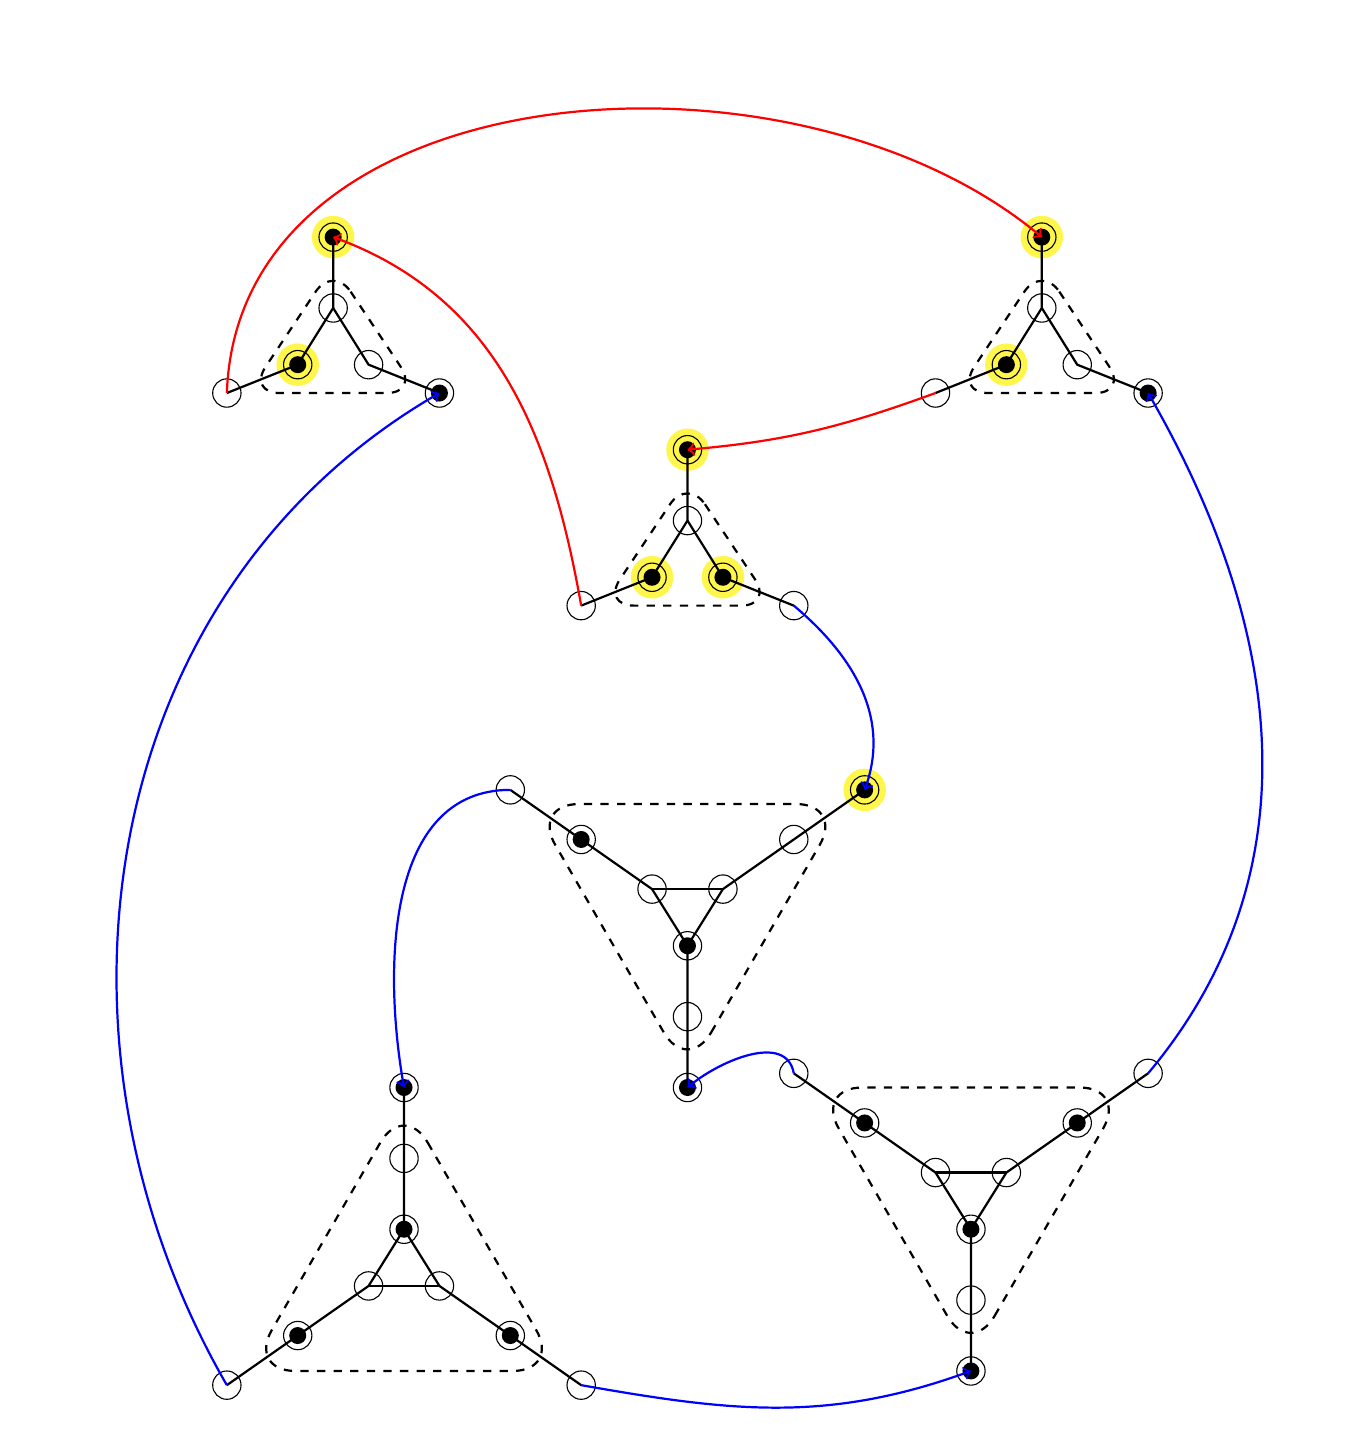
\begin{tikzpicture}[scale=0.9]
      %%%%%%%%%%%% AND 1 %%%%%%%%%%%%
      \def\ver{0.12} %size of a vertex
      \def\xa{-1}
      \def\ya{0}
      % Highlight change
      \draw[fill=yellow, opacity=.7, draw=none] (\xa,\ya+1) circle (0.3cm);
      \draw[fill=yellow, opacity=.7, draw=none] (\xa-0.5,\ya-0.8) circle (0.3cm);
      %graph G
      \draw (\xa,\ya) circle (0.2cm);          %v1 no fill
      \draw (\xa,\ya+1) circle (0.2cm);        %v2 no fill
      \draw (\xa+0.5,\ya-0.8) circle (0.2cm);  %v4 no fill
      \draw (\xa-0.5,\ya-0.8) circle (0.2cm);  %v3 no fill
      \draw (\xa-1.5,\ya-1.2) circle (0.2cm);  %v5 no fill
      \draw (\xa+1.5,\ya-1.2) circle (0.2cm);  %v6 no fill
      % Tokens
      \path[fill] (\xa,\ya+1) circle (\ver);         %v2
      \path[fill] (\xa-0.5,\ya-0.8) circle (\ver);   %v3
      \path[fill] (\xa+1.5,\ya-1.2) circle (\ver);   %v6
      %labels
      \draw[thick] (\xa,\ya+1)--(\xa,\ya)--(\xa-0.5,\ya-0.8)--(\xa-1.5,\ya-1.2);
      \draw[thick] (\xa,\ya)--(\xa+0.5,\ya-0.8)--(\xa+1.5,\ya-1.2);
      \path[draw, thick, dashed, rounded corners=4mm] (\xa,\ya+0.6)--(\xa+1.2,\ya-1.2)--(\xa-1.2,\ya-1.2)--cycle;

      %%%%%%%%%%%% AND 2 %%%%%%%%%%%%
      \def\ver{0.12} %size of a vertex
      \def\xb{4}
      \def\yb{-3}
      % Highlight change
      \draw[fill=yellow, opacity=.7, draw=none] (\xb,\yb+1) circle (0.3cm);
      \draw[fill=yellow, opacity=.7, draw=none] (\xb-0.5,\yb-0.8) circle (0.3cm);
      \draw[fill=yellow, opacity=.7, draw=none] (\xb+0.5,\yb-0.8) circle (0.3cm);
      %graph G
      \draw (\xb,\yb) circle (0.2cm);          %v1 no fill
      \draw (\xb,\yb+1) circle (0.2cm);        %v2 no fill
      \draw (\xb+0.5,\yb-0.8) circle (0.2cm);  %v4 no fill
      \draw (\xb-0.5,\yb-0.8) circle (0.2cm);  %v3 no fill
      \draw (\xb-1.5,\yb-1.2) circle (0.2cm);  %v5 no fill
      \draw (\xb+1.5,\yb-1.2) circle (0.2cm);  %v6 no fill
      \path[fill] (\xb,\yb+1) circle (\ver);         %v2
      \path[fill] (\xb-0.5,\yb-0.8) circle (\ver); %v3
      \path[fill] (\xb+0.5,\yb-0.8) circle (\ver); %v4
      %labels
      \draw[thick] (\xb,\yb+1)--(\xb,\yb)--(\xb-0.5,\yb-0.8)--(\xb-1.5,\yb-1.2);
      \draw[thick] (\xb,\yb)--(\xb+0.5,\yb-0.8)--(\xb+1.5,\yb-1.2);
      \path[draw, thick, dashed, rounded corners=4mm] (\xb,\yb+0.6)--(\xb+1.2,\yb-1.2)--(\xb-1.2,\yb-1.2)--cycle;

      %%%%%%%%%%%% AND 3 %%%%%%%%%%%%
      \def\ver{0.12} %size of a vertex
      \def\xc{9}
      \def\yc{0}
      % Highlight change
      \draw[fill=yellow, opacity=.7, draw=none] (\xc,\yc+1) circle (0.3cm);
      \draw[fill=yellow, opacity=.7, draw=none] (\xc-0.5,\yc-0.8) circle (0.3cm);
      %graph G
      \draw (\xc,\yc) circle (0.2cm);          %v1 no fill
      \draw (\xc,\yc+1) circle (0.2cm);        %v2 no fill
      \draw (\xc+0.5,\yc-0.8) circle (0.2cm);  %v4 no fill
      \draw (\xc-0.5,\yc-0.8) circle (0.2cm);  %v3 no fill
      \draw (\xc-1.5,\yc-1.2) circle (0.2cm);  %v5 no fill
      \draw (\xc+1.5,\yc-1.2) circle (0.2cm);  %v6 no fill
      \path[fill] (\xc,\yc+1) circle (\ver);         %v2
      \path[fill] (\xc-0.5,\yc-0.8) circle (\ver);   %v3
      \path[fill] (\xc+1.5,\yc-1.2) circle (\ver);   %v6
      %labels
      \draw[thick] (\xc,\yc+1)--(\xc,\yc)--(\xc-0.5,\yc-0.8)--(\xc-1.5,\yc-1.2);
      \draw[thick] (\xc,\yc)--(\xc+0.5,\yc-0.8)--(\xc+1.5,\yc-1.2);
      \path[draw, thick, dashed, rounded corners=4mm] (\xc,\yc+0.6)--(\xc+1.2,\yc-1.2)--(\xc-1.2,\yc-1.2)--cycle;

      %%%%%%%%%%%% OR 1 %%%%%%%%%%%%
      \def\ver{0.12} %size of a vertex
      \def\xd{0}
      \def\yd{-13}
      %G_1
      \draw (\xd,\yd+2) circle (0.2cm);         %v9
      \draw (\xd,\yd) circle (0.2cm);           %v1
      \draw (\xd+0.5,\yd-0.8) circle (0.2cm);   %v4
      \draw (\xd-0.5,\yd-0.8) circle (0.2cm);   %v3
      \draw (\xd,\yd+1) circle (0.2cm);         %v2
      \draw (\xd-1.5,\yd-1.5) circle (0.2cm);   %v5
      \draw (\xd+1.5,\yd-1.5) circle (0.2cm);   %v6
      \draw (\xd-2.5,\yd-2.2) circle (0.2cm);     %v7
      \draw (\xd+2.5,\yd-2.2) circle (0.2cm);     %v8

      \path[fill] (\xd,\yd+2) circle (\ver);         %v0
      \path[fill] (\xd,\yd) circle (\ver);           %v1
      \path[fill] (\xd-1.5,\yd-1.5) circle (\ver);   %v5
      \path[fill] (\xd+1.5,\yd-1.5) circle (\ver);   %v6
      %labels
      \draw[thick] (\xd,\yd+2)--(\xd,\yd+1)--(\xd,\yd)--(\xd-0.5,\yd-0.8)--(\xd-1.5,\yd-1.5)--(\xd-2.5,\yd-2.2);
      \draw[thick] (\xd,\yd)--(\xd+0.5,\yd-0.8)--(\xd+1.5,\yd-1.5)--(\xd+2.5,\yd-2.2);
      \draw[thick] (\xd-0.5,\yd-0.8)--(\xd+0.5,\yd-0.8);
      \path[draw, thick, dashed, rounded corners=6mm] (\xd,\yd+1.8)--(\xd+2.2,\yd-2)--(\xd-2.2,\yd-2)--cycle;

      %%%%%%%%%%%% OR 2 %%%%%%%%%%%%
      \def\ver{0.12} %size of a vertex
      \def\xe{4}
      \def\ye{-9}
      % Highlight change
      \draw[fill=yellow, opacity=.7, draw=none] (\xe+2.5,\ye+2.2) circle (0.3cm);
      %G_1
      \draw (\xe,\ye-2) circle (0.2cm);         %v9
      \draw (\xe,\ye) circle (0.2cm);           %v1
      \draw (\xe+0.5,\ye+0.8) circle (0.2cm);   %v4
      \draw (\xe-0.5,\ye+0.8) circle (0.2cm);   %v3
      \draw (\xe,\ye-1) circle (0.2cm);         %v2
      \draw (\xe-1.5,\ye+1.5) circle (0.2cm);   %v5
      \draw (\xe+1.5,\ye+1.5) circle (0.2cm);   %v6
      \draw (\xe-2.5,\ye+2.2) circle (0.2cm);     %v7
      \draw (\xe+2.5,\ye+2.2) circle (0.2cm);     %v8

      \path[fill] (\xe,\ye-2) circle (\ver);         %v9
      \path[fill] (\xe,\ye) circle (\ver);           %v1
      \path[fill] (\xe-1.5,\ye+1.5) circle (\ver);   %v5
      \path[fill] (\xe+2.5,\ye+2.2) circle (\ver);   %v8
      %labels
      \draw[thick] (\xe,\ye-2)--(\xe,\ye-1)--(\xe,\ye)--(\xe-0.5,\ye+0.8)--(\xe-1.5,\ye+1.5)--(\xe-2.5,\ye+2.2);
      \draw[thick] (\xe,\ye)--(\xe+0.5,\ye+0.8)--(\xe+1.5,\ye+1.5)--(\xe+2.5,\ye+2.2);
      \draw[thick] (\xe-0.5,\ye+0.8)--(\xe+0.5,\ye+0.8);
      \path[draw, thick, dashed, rounded corners=6mm] (\xe,\ye-1.8)--(\xe+2.2,\ye+2)--(\xe-2.2,\ye+2)--cycle;

      %%%%%%%%%%%% OR 3 %%%%%%%%%%%%
      \def\ver{0.12} %size of a vertex
      \def\xf{8}
      \def\yf{-13}
      %G_1
      \draw (\xf,\yf-2) circle (0.2cm);         %v9
      \draw (\xf,\yf) circle (0.2cm);           %v1
      \draw (\xf+0.5,\yf+0.8) circle (0.2cm);   %v4
      \draw (\xf-0.5,\yf+0.8) circle (0.2cm);   %v3
      \draw (\xf,\yf-1) circle (0.2cm);         %v2
      \draw (\xf-1.5,\yf+1.5) circle (0.2cm);   %v5
      \draw (\xf+1.5,\yf+1.5) circle (0.2cm);   %v6
      \draw (\xf-2.5,\yf+2.2) circle (0.2cm);     %v7
      \draw (\xf+2.5,\yf+2.2) circle (0.2cm);     %v8

      \path[fill] (\xf,\yf-2) circle (\ver);         %v0
      \path[fill] (\xf,\yf) circle (\ver);           %v1
      \path[fill] (\xf-1.5,\yf+1.5) circle (\ver);   %v5
      \path[fill] (\xf+1.5,\yf+1.5) circle (\ver);   %v6
      %labels
      \draw[thick] (\xf,\yf-2)--(\xf,\yf-1)--(\xf,\yf)--(\xf-0.5,\yf+0.8)--(\xf-1.5,\yf+1.5)--(\xf-2.5,\yf+2.2);
      \draw[thick] (\xf,\yf)--(\xf+0.5,\yf+0.8)--(\xf+1.5,\yf+1.5)--(\xf+2.5,\yf+2.2);
      \draw[thick] (\xf-0.5,\yf+0.8)--(\xf+0.5,\yf+0.8);
      \path[draw, thick, dashed, rounded corners=6mm] (\xf,\yf-1.8)--(\xf+2.2,\yf+2)--(\xf-2.2,\yf+2)--cycle;

      %%%%%%%%%%% EDGES %%%%%%%%%
      \draw [-, red, thick, arrows={->[scale=3,red]}] (\xa-1.5,\ya-1.2) to [out=88,in=140] (\xc,\yc+1);              % AND 3  -- AND 1
      \draw [-, red, thick, arrows={->[scale=3,red]}] (\xb-1.5,\yb-1.2)  to [out=100,in=340] (\xa,\ya+1);             % AND 1  -- AND 2
      \draw [-, red, thick, arrows={->[scale=3,red]}] (\xc-1.5,\yc-1.2) to [out=200,in=5] (\xb,\yb+1);              % AND 2  -- AND 3
      \draw [-, blue, thick, arrows={->[scale=3,blue]}] (\xd-2.5,\yd-2.2) to [out=120,in=210] (\xa+1.5,\ya-1.2);     % OR 1  -- AND 1
      \draw [-, blue, thick, arrows={->[scale=3,blue]}] (\xd+2.5,\yd-2.2) to [out=350,in=200] (\xf,\yf-2);            % OR 1  -- OR 3
      \draw [-, blue, thick, arrows={->[scale=3,blue]}] (\xf-2.5,\yf+2.2) to [out=100,in=40] (\xe,\ye-2);            % OR 3  -- OR 2
      \draw [-, blue, thick, arrows={->[scale=3,blue]}] (\xe-2.5,\ye+2.2) to [out=180,in=100] (\xd,\yd+2);            % OR 2  -- OR 1
      \draw [-, blue, thick, arrows={->[scale=3,blue]}] (\xf+2.5,\yf+2.2) to [out=50,in=300] (\xc+1.5,\yc-1.2);            % OR 3  -- AND 3
      \draw [-, blue, thick, arrows={->[scale=3,blue]}] (\xb+1.5,\yb-1.2) to [out=320,in=70] (\xe+2.5,\ye+2.2);            % OR 2  -- AND 2
    \end{tikzpicture}
  \end{scaletikzpicturetowidth}
  \caption{Sliding Tokens vertex gadgets.}
  \label{fig:output_instance_final}
\end{figure}



